\section{Modelling Security Properties with Automata}\label{SecMVA}

This section formally defines our format of security automata. They
are particularly suited for monitoring, because transitions can depend
on the state of the monitored program. We call them
\marginnote{\small MH: Multi-Variable Automata not very good/catchy name
 AT: What about: Property Automata, Security Automata (or more precisely
 Safety Automata), Pushdown Automata, just Automata or just Property.
 I like Property Automata}
\emph{Multi-Variable Automata} (MVA). %because their states are defined
%by a set of variables.
Transitions between states are labelled with guards, events and a list
of actions. The event specifies the method whose entry and/or exit is
being monitored, with a distinction between normal and exceptional
exits.  The guard describes the conditions under which the transition
can be applied. It depends on
\begin{inparaenum}[(\itshape i\upshape)]
\item the automaton state,
\item the state of the program that is being monitored, and
\item the argument of the method, in case the event is method entry;
the result of the method, in case the event is normal method exit; or
the exception with which the method returns, in case the event is
exceptional method exit.
\end{inparaenum}
Each action describes how the automaton state is updated by the transition.
\marginnote{\small MH: conditions on guards/actions?
 AT: I wouldn't mention them we have the specification for all the details.}

MVA and programs share the definitions of values, types and exceptions, denoted
\Val, \Type and \Excpt, respectively. They are defined by the following grammar,
where \(\mathbb{B}\) and \(\mathbb{Z}\) denote the standard sets of booleans
and integers, respectively\footnote{We will
use a PVS-like notation to declare abstract data types and records
(enclosed by \(\opr\) and \(\clr\)). Further, if \(x\) is a
record with field \textsf{y}, we use \(x.\mathsf{y}\) to access field
\textsf{y}, and \(x \opri\mathsf{y} := z\clri\) to denote the record
\(x\) with the field \textsf{y} updated to \(z\).}.
\[{\small
\begin{array}{rcl}
\Val & = & \B(b : \mathbb{B}) \mid \I(i : \mathbb{Z}) \mid \Null \mid
\R(i : \mathbb{Z}) \mid \One \mid \bot\\
\Type & = & \Bool \mid \Int \mid \Ref \mid \Void\\
\Excpt & = & \Throwable \mid \NullPointer \mid \JMLExc
\end{array}}
\]
Notice that there is a special type \(\Void\), inhabited by \(\One\)
to model methods without results. Reference values contain a number,
which can be considered as the location where the object is stored;
\(\bot\) is used to denote the outcome of an undefined expression.
Throughout, we assume that \(\CP\) and \(\Name\) are infinite, but
enumerable nonempty sets of control points and names, respectively.
% We assume that \(\Name\) contains the special names \textsf{this}.


An MVA consists of
\begin{inparaenum}[(\itshape i\upshape)]
\item a name,
\item a class name, to specify which class is being monitored,
\item a finite set of control points,
\item an initial control point,
\item a set of events, to specify which methods are being monitored,
\item a set of MVA variable declarations, to describe
the internal state of the automaton
\item a set of program variable declarations, to specify which
program variables will be inspected by the monitor, and
\item a set of transitions.
\end{inparaenum}
Transitions go from source to target control points. They are labelled
with events, where an event is a tuple of an event type (entry, exit
or exceptional exit) and a method name, guards and a list of
actions. Each action assigns the result of an expression (containing
both program and MVA variables) to an MVA variable. MVA variables
declarations are the same as program field declarations (defined
below), while program variable declarations in the MVA have the same
format as local variable declarations in a program (\emph{i.e.}, they
are not explicitly initialised in the monitor, their value is retrieved from
the program state.). Figure~\ref{FigMVAForm} shows the
main types of the MVA definition.
%% This is already said
% (the types of \FieldDecl and
% \LocalVarDecl will also be used in the abstract syntax of programs).

\begin{figure}[t]
\[{\small
\begin{array}{rcl}
\FieldDecl & = \opr & \type : \Type, \name : \Name, \init : \Val
\clr \\
\LocalVarDecl & = \opr & \type : \Type, \name : \Name \clr \\
\EVENT & = \opr & \etype : (\entry \mid \exit \mid \excexit),
                 \mname : \Name \clr\\
\TRANS & = \opr & \scp, \tcp : \CP, \event : \EVENT, \\
& &
\guard : \MVAstate \times \Pstate \times (\Val \mid \Excpt) \rightarrow \mathbb{B}, \\
&& \action : (\opr \target : \Name, \expr : \Expr \clr)^* \clr\\
\MVA & = \opr & \name, \clname : \Name, \cps : \setof{\CP},
            \init : \CP, \evs : \setof{\EVENT},\\
     &   &  \vdsA : \setof{\FieldDecl}, \vdsP : \setof{\LocalVarDecl},\\
     &   &  \trans : \setof{\TRANS} \clr
\end{array}}
\]
\caption{Formal Definition of MVA}\label{FigMVAForm}
\end{figure}

We require an MVA to be \emph{deterministic}, \emph{i.e.}, for every
source control point and event there is always at most one guard that
holds. Notice that it is not obvious how to transform a
non-deterministic MVA into a deterministic one, because the actions
made by the overlapping transitions might be different.
% We believe that this is a realistic restriction, and that most important
% security properties can be expressed as deterministic MVAs.

An MVA is \emph{total} if there is always exactly one guard that holds
for a given source control point and event, otherwise it is
\emph{partial}. Every deterministic MVA can be completed into a total
one (by function \complete): add a special control state
\halted, together with transitions for every control point and every event
to this \halted control point, where the guard is the negation of the
disjunction of all other guards for this control point and event, and
in addition, add unconditional transitions from \halted to \halted
for every possible event.

%\marginnote{MH: Should we give formal definition of \emph{complete}?}

We define a collection of constraints to say that an MVA is
\emph{wellformed}, such as:
\begin{inparaenum}[(\itshape i\upshape)]
% \item the monitor variable names do not overlap with the reserved
% words,
% \item the program variable names that are used are unique,
\item variable names are unique and are not reserved words,
\item guards do not have side-effects,
\item guards and actions only use declared variables, and
\item control points and events used in transitions are declared.
% \item transitions range between declared control points and are
% labelled with declared events.
\end{inparaenum}

%Formally:
%\[
%\begin{array}[t]{l}
%\mathsf{complete}(a) =
%\begin{array}[t]{l}
%a \mathsf{with} (\#
%\begin{array}[t]{l}
%\cps := a.\cps \cup {\halted},
%\trans := a.\trans \cup complete(a.\trans)
%\end{array}
%\#)
%\end{array}
%\mathsf{complete}(T) =
%\{ (\# \scp := q,
%       \tcp := \halted,
%       \guard := \lambda \sigma_A \sigma_P v.
%\end{array}
%\]

% \paragraph{MVA Transitions}
The state of an MVA consists of a current control point, and the store of
automaton variables (the program store is not part of the automaton state).
\[{\small
\MVAstate = \opr \cp : \CP, \stA : \Store \clr}
\]
Given an MVA \(a\), the transition function \(\Delta_a\)
describes how given a program store and an event, \(a\) changes its
internal state (where \(\chooseop\) is the arbitrary choice operator,
and \textsf{apply} is a function that updates the automaton store
according to the list of actions in the obvious way).
\[{\small
\begin{array}{l}
\Delta_a  :  \MVAstate \times \Pstate \times \EVENT \times (\Val \mid
\Excpt) \hookrightarrow
\MVAstate\\
\Delta_a(\sigma_A, \sigma_P, e, v) = \\
\quad
\begin{array}[t]{l}
\mathsf{let\ }t = \chooseop(\{t\in \trans(a)\mid
  \begin{array}[t]{l}
     t.\scp = \sigma_A.\cp \wedge t.\event = e \wedge \\
     t.\guard(\sigma_A.\stA, \sigma_P.\fvs.\st, v)\}) \mathsf{\ in}
  \end{array}\\
\quad \opri \cp := t.\tcp, \stA := \mathit{apply}(t.\action,
\sigma_A.\stA) \clri
\end{array}

\end{array}}
\]
In a total MVA $a$, the transition function \(\Delta_a\) is total.
A partial automaton gets stuck on a certain input if and only if the
complete MVA reaches the state \halted.

\begin{equation}\label{MVAcompletionProp}
\Delta_a(\sigma_A, \sigma_P, e, v) = \perp \Leftrightarrow
\cp (\Delta_{\complete(a)}(\sigma_A, \sigma_P, e, v)) = \halted
\end{equation}


\paragraph{Example}
The following MVA\footnote{Where \(\actskip\) denotes an empty sequence.}
encodes the property described in Figure~\ref{FigExample}.
% Recall the example security automaton in Figure~\ref{FigExample},
% expressing that the method \texttt{sendSMS} can
% be called at most \(N\) times in between calls to a \texttt{reset}
% method. This property is formally described by the following
% automaton\footnote{Where \(\actskip\) denotes an empty sequence.}.
\[
\small{
\hspace{-0.3em}
\begin{array}[t]{l}
\opri
\begin{array}[t]{l}
\name := \textrm{LimitSMS}, \clname := \texttt{Messaging},
\cps := \{s_1, s_2\},
\init := s_1,\\
\evs :=
\begin{array}[t]{l}
\{ \opri \etype := e, \mname := \texttt{sendSMS} \clri \mid e \in \opri \entry,
\exit, \excexit \} \:\cup \\
\{ \opri \etype := \exit, \mname := \texttt{reset} \clri\},
\end{array}
\\
\vdsA := \{\opri \name := n, \type := \Int, \init := 0 \clri\},
\vdsP := \emptyset,\\
\trans := \{
\begin{array}[t]{l}
\opri
 \begin{array}[t]{l}
\scp := s_1, \tcp := s_2, \\
             \event := \opri \etype := \entry,
                             \mname := \texttt{sendSMS} \clri, \\
             \guard := \lambda(\sigma_A, \sigma_P, v). n(\sigma_A) < N,
             \action := \actskip
            \clri,
\end{array}\\
\opri
 \begin{array}[t]{l}
\scp := s_2, \tcp := s_1, \\
             \event := \opri \etype := \exit,
                             \mname := \texttt{sendSMS} \clri, \\
             \guard := \lambda(\sigma_A, \sigma_P, v). \ttt,
             \action := [\opri \target := n, \expr := n + 1 \clri]
            \clri,
\end{array}\\
\opri
 \begin{array}[t]{l}
\scp := s_2, \tcp := s_1, \\
             \event := \opri \etype := \excexit,
                             \mname := \texttt{sendSMS} \clri, \\
             \guard := \lambda(\sigma_A, \sigma_P, v). \ttt,
             \action := \actskip
            \clri,
\end{array}\\
\opri
\begin{array}[t]{l}
\scp := s_1, \tcp := s_1, \\
             \event := \opri \etype := \exit, \mname := \texttt{reset}
\clri, \\
             \guard := \lambda(\sigma_A, \sigma_P, v). \ttt,
             \action := [\opri \target := n, \expr := 0 \clri]
           \clri \} \clri
\end{array}
\end{array}
\end{array}\\
\end{array}
}\]

% Completion adds the following transitions to the automaton in
% Figure~\ref{FigExample}: from \(s_1\) to \halted, for the event
% \entry(\texttt{sendSMS}), with guard \(n \geq N\); and for the events
% \exit(\texttt{sendSMS}) and \excexit(\texttt{sendSMS}), with guard \ttt;
% from \(s_2\) to \halted, for the events \entry(\texttt{sendSMS}) and
% \exit(\texttt{reset}), with guard \ttt, from \halted to \halted, for
% all events and with guard \ttt.
Figure~\ref{FigCompleteMVA} shows the completed MVA.

\psfrag{s1}{\tiny{\(s_1\)}}
\psfrag{s2}{\tiny{\(s_2\)}}
\psfrag{exit(sendSMS)?true -> n := n + 1;}
{\begin{tabular}{l}
\tiny{\exit(\texttt{SendSMS})?\ttt}\vspace*{-.8em}\\
\tiny{\(\rightarrow\)\texttt{n := n + 1};}
\end{tabular}}
\psfrag{exitE(sendSMS)?true -> ;}
{\begin{tabular}{l}
\tiny{\excexit(\texttt{sendSMS})?\ttt \(\rightarrow\)}%\vspace*{-.8em}\\
\tiny{\actskip;}
\end{tabular}}
\psfrag{exit(reset)?true -> n := 0;}
{\begin{tabular}{l}
\tiny{\exit(\texttt{reset})?\ttt \(\rightarrow\)}\vspace*{-.8em} \\
\tiny{\texttt{n :=} 0;}
\end{tabular}}
\psfrag{entry(sendSMS)? n<N -> ;}
{\begin{tabular}{l}
\tiny{\entry(\texttt{sendSMS})? \texttt{n} \(<\) \texttt{N} \(\rightarrow\)} %\vspace*{-.8em} \\
\tiny{\actskip;}
\end{tabular}}
\psfrag{entry(sendSMS)?true -> ;}
{\tiny{\entry(\texttt{sendSMS})?\ttt \(\rightarrow\)\actskip}}
\psfrag{exit(reset)?true -> ;}
{\tiny{\exit(\texttt{reset})?\ttt \(\rightarrow\)\actskip}}
\psfrag{exit(sendSMS)?true -> ;}
{\tiny{\exit(\texttt{sendSMS})?\ttt \(\rightarrow\)\actskip}}
\psfrag{exitE(sendSMS)?true -> ;}
{\tiny{\excexit(\texttt{sendSMS})?\ttt \(\rightarrow\)\actskip}}
\psfrag{entry(sendSMS)?n >= N -> ;}
{\tiny{\entry(\texttt{sendSMS})?\texttt{n} \(\geq\) \texttt{N}
\(\rightarrow\)\actskip}}
\psfrag{halted}{\tiny{\halted}}

\begin{figure}[t]
\begin{center}
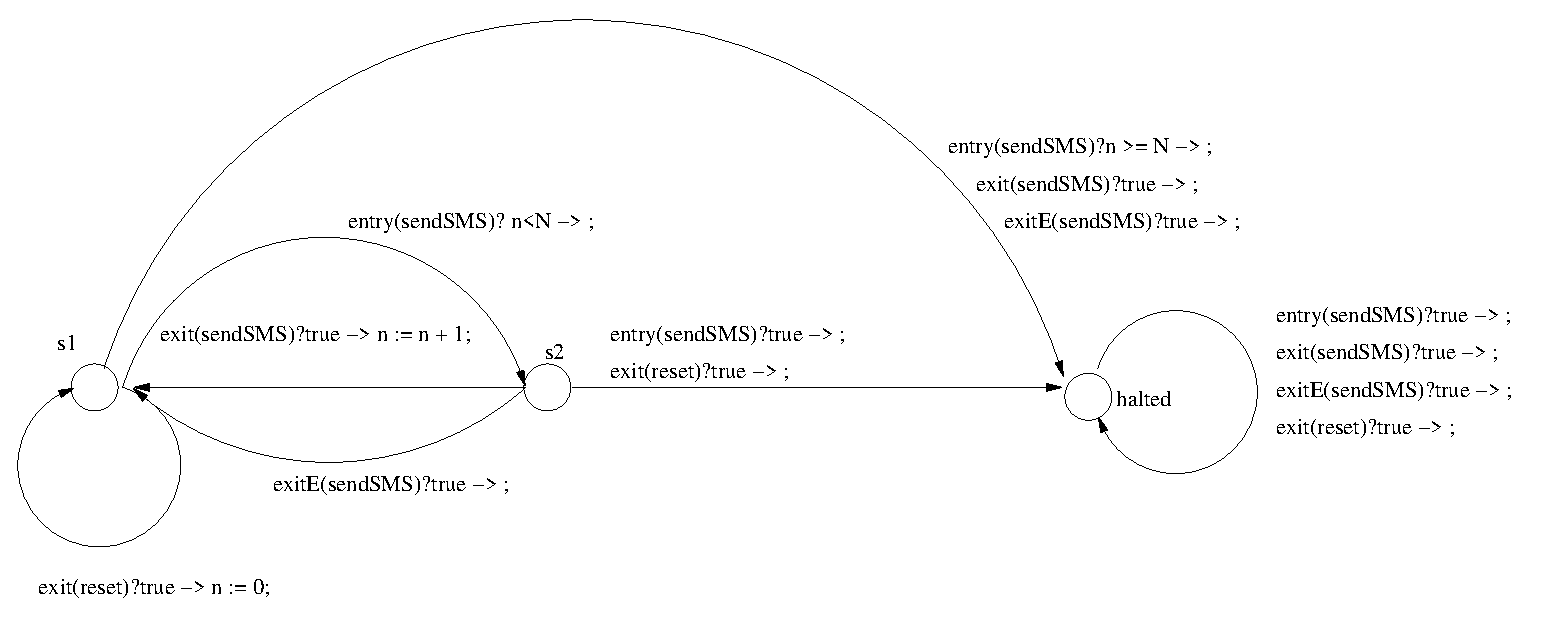
\epsfig{file=completed_alt.eps, width=8cm}
\end{center}
\label{FigCompleteMVA}
\caption{Automaton of Figure~\ref{FigExample}, after completion}
\end{figure}
